\paperchapter{October 2010}{October 2010}{A}{60}{GSET 2010}
\keytable{\kcell{1}{C} & \kcell{2}{C} & \kcell{3}{D} & \kcell{4}{D} & \kcell{5}{D} & \kcell{6}{A} & \kcell{7}{B} & \kcell{8}{C} & \kcell{9}{A} & \kcell{10}{C} \\
\kcell{11}{C} & \kcell{12}{D} & \kcell{13}{B} & \kcell{14}{C} & \kcell{15}{B} & \kcell{16}{A} & \kcell{17}{A} & \kcell{18}{B} & \kcell{19}{B} & \kcell{20}{A} \\
\kcell{21}{C} & \kcell{22}{B} & \kcell{23}{A} & \kcell{24}{B} & \kcell{25}{B} & \kcell{26}{B} & \kcell{27}{D} & \kcell{28}{A} & \kcell{29}{D} & \kcell{30}{C} \\
\kcell{31}{A} & \kcell{32}{B} & \kcell{33}{D} & \kcell{34}{C} & \kcell{35}{A} & \kcell{36}{D} & \kcell{37}{A} & \kcell{38}{C} & \kcell{39}{B} & \kcell{40}{D} \\
\kcell{41}{C} & \kcell{42}{B} & \kcell{43}{D} & \kcell{44}{C} & \kcell{45}{C} & \kcell{46}{C} & \kcell{47}{X} & \kcell{48}{D} & \kcell{49}{B} & \kcell{50}{B} \\
\kcell{51}{C} & \kcell{52}{C} & \kcell{53}{D} & \kcell{54}{D} & \kcell{55}{C} & \kcell{56}{B} & \kcell{57}{C} & \kcell{58}{A} & \kcell{59}{D} & \kcell{60}{B}}
\begin{question}{1}
{Which of the following statements defines education best ?\par}
\optstwo{Education is a means of social change}{Education imparts useful knowledge}{It prepares autonomous human beings}{It generates a lot of employment}
\answer{C}{It prepares autonomous human beings}
\begin{explain}
The best definition of education is that it \textbf{prepares autonomous human beings}: individuals who think, judge and act independently and responsibly. Social change, useful knowledge and employment are only by-products.
\end{explain}
\end{question}

\begin{question}{2}
{Semester system is recommended as it is considered to:\par}
\optsone{help students learn more efficiently and be regular}{reduce examination orientedness and increase emphasis on learning}{provide scope for continual appraisal and on course correction in teaching-learning process}{allow for more creative ways of teaching}
\answer{C}{provide scope for continual appraisal and on course correction in teaching-learning process}
\begin{explain}
The semester system provides \textbf{scope for continual appraisal}: frequent assessment, feedback and course correction within shorter learning units, per the official key.
\end{explain}
\end{question}

\begin{question}{3}
{It is said that teachers must enable students to own the responsibility for learning. This means teachers\par}
\optsone{have reduced responsibility of learning}{assign learning tasks to students}{ask students to study on their own}{must help students to evolve one's own ways of learning}
\answer{D}{must help students to evolve one's own ways of learning}
\begin{explain}
Making students own responsibility for learning means the teacher \textbf{helps students evolve their own ways of learning}, so that they become self-directed, independent learners.
\end{explain}
\end{question}

\begin{question}{4}
{At higher education stage emphasis needs to be on, not only 'what' and 'how much' is learned by students but 'how' and 'how well' they learn. This idea is expressed at present as:\par}
\optstwo{Learning to know}{Learning to live}{Learning to do}{Learning to learn}
\answer{D}{Learning to learn}
\begin{explain}
Emphasis on ``how'' and ``how well'' students learn reflects the idea of \textbf{learning to learn}, i.e.\ developing metacognition and lifelong learning skills. (Compare the Delors Report's four pillars: learning to know, to do, to live together, to be.)
\end{explain}
\end{question}

\begin{question}{5}
{The current thinking of assessing students only at the end of the term is less relevant as it :\par}
\optsone{reveals student's learning in respect of subject matter}{concerns with how accurately one recollects the subject matter}{may reveal 'temporary learning' and not beyond}{assesses student learning on 'what is asked' rather than 'what is learned' even beyond subject matter}
\answer{D}{assesses student learning on 'what is asked' rather than 'what is learned' even beyond subject matter}
\begin{explain}
Assessment only at the end of term is less useful because it may capture \textbf{temporary learning} (crammed and soon forgotten) rather than lasting understanding. Continuous assessment gives a truer picture.
\end{explain}
\end{question}

\begin{question}{6}
{Arrange the following from the least difficult to most difficult:\newline (1) Teaching of processes\newline (2) Teaching of values\newline (3) Teaching of concepts\newline (4) Teaching of thinking skills\par}
\optstwo{(1), (3), (4), (2)}{(2), (4), (3), (1)}{(1), (3), (2), (4)}{(1), (2), (3), (4)}
\answer{A}{(1), (3), (4), (2)}
\begin{explain}
From least to most difficult: teaching \textbf{processes (1)} $\rightarrow$ \textbf{concepts (3)} $\rightarrow$ \textbf{thinking skills (4)} $\rightarrow$ \textbf{values (2)}. Values are the hardest because they involve the affective domain and must be internalised.
\end{explain}
\end{question}

\begin{question}{7}
{Recently a separate Board has been established to monitor all \ldots{} education institutions in Gujarat.\par}
\optsfour{legal}{technical}{medical}{professional}
\answer{B}{technical}
\begin{explain}
Gujarat set up a separate board (Admission Committee for Professional Courses / the regulatory board under the Gujarat Professional \textbf{Technical} Educational Colleges or Institutions Act, 2007) to regulate admissions and fees of \textbf{technical} education institutions, per the key.
\end{explain}
\end{question}

\begin{question}{8}
{The increasing number of entrants into higher education has necessitated changes in our views of teaching learning. Some progressive institutions have faced this through the adoption of multimedia for teaching-learning. This means, the use of \ldots{} for teaching learning.\par}
\optsone{lecture-cum-discussion, practical work}{face to face, distance and open learning (ODL) systems}{ODL, face to face, satellite and web based modes}{self-learning, ICT based, ODL}
\answer{C}{ODL, face to face, satellite and web based modes}
\begin{explain}
Progressive institutions cope with rising numbers by using multimedia across \textbf{ODL, face-to-face, satellite and web-based modes}, i.e.\ blended and multi-mode delivery.
\end{explain}
\end{question}

\begin{question}{9}
{Apart from specialisation in one's subject areas, products of higher education are also expected to be \ldots{} in the context of national development.\par}
\optsone{sensitive and proactive towards emerging concerns and issues}{responsible workers in one's institution}{aware of the economic changes especially the job market}{tolerant to the negative forces}
\answer{A}{sensitive and proactive towards emerging concerns and issues}
\begin{explain}
Graduates are expected to be \textbf{sensitive and proactive towards emerging concerns and issues} of society and the nation, not merely job-seekers.
\end{explain}
\end{question}

\begin{question}{10}
{To ensure quality maintenance in universities and colleges guidelines and regulations are periodically prepared by the \ldots{} at the national level.\par}
\optsone{National Assessment and Accreditation Council (NAAC)}{National Council for Educational Research and Training (NCERT)}{University Grants Commission (UGC)}{National Institute of Advanced Study (NIAS)}
\answer{C}{University Grants Commission (UGC)}
\begin{explain}
The \textbf{UGC} frames regulations and guidelines for maintaining standards in universities and colleges (UGC Act, 1956, Section 12). NAAC only assesses and accredits.
\end{explain}
\end{question}

\begin{question}{11}
{The open university at the national level in India is known as:\par}
\optsone{Indian General National Open University}{Integrated Governmental National Open University}{Indira Gandhi National Open University}{Iswarbhai Gordhanbhai National Open University}
\answer{C}{Indira Gandhi National Open University}
\begin{explain}
The national open university is \textbf{Indira Gandhi National Open University (IGNOU)}, New Delhi (1985).
\end{explain}
\end{question}

\begin{question}{12}
{Three kinds of universities in India are:\par}
\optsone{State Universities, Central Universities, Affiliating Universities}{Unitary Universities, Technical Universities, General Education Universities}{State Universities, Central Universities, Private Universities}{Central Universities, State Universities, Deemed Universities}
\answer{D}{Central Universities, State Universities, Deemed Universities}
\begin{explain}
Per the key, the three kinds are \textbf{State Universities, Central Universities and Deemed-to-be Universities} (with private universities being added later).
\end{explain}
\end{question}

\begin{question}{13}
{A condition or characteristic that can take on different values or categories is called:\par}
\optstwo{a constant}{a variable}{a cause and effect relationship}{a descriptive relationship}
\answer{B}{a variable}
\begin{explain}
A characteristic that can take different values or categories is a \textbf{variable}; one that cannot vary is a constant.
\end{explain}
\end{question}

\begin{question}{14}
{A researcher wants to find out the relationship between gender and intelligence among high school students. This would be :\par}
\optstwo{a Case Study}{a Developmental Study}{a Survey Study}{an Experimental Study}
\answer{C}{a Survey Study}
\begin{explain}
Studying the relationship between gender and intelligence in a population of students, as they exist without manipulation, is a \textbf{survey (descriptive--correlational) study}.
\end{explain}
\end{question}

\begin{question}{15}
{The best graphical way to present data related to different levels of a certain variable is:\par}
\optstwo{pictogram}{pie chart}{histogram}{frequency polygon}
\answer{B}{pie chart}
\begin{explain}
Per the key, a \textbf{pie chart} best shows how a whole is divided among the different levels (categories) of a variable.
\end{explain}
\end{question}

\begin{question}{16}
{In simple terms 'reliability' is the:\par}
\optsone{consistency of scores on tests}{appropriateness of interpretation based on test scores}{ways in which people are the same}{rank order of participants on some measure}
\answer{A}{consistency of scores on tests}
\begin{explain}
\textbf{Reliability} is the \textbf{consistency} (stability) of test scores. Appropriateness of interpretations is \emph{validity}.
\end{explain}
\end{question}

\begin{question}{17}
{A researcher was interested in studying why learning of new maths was not effective in schools during 1990s. For this, he interviewed several teachers who had taught new maths at that time. These teachers were \ldots{} for his study.\par}
\optstwo{primary sources}{secondary sources}{external critics}{internal critics}
\answer{A}{primary sources}
\begin{explain}
Teachers who personally taught the new maths are eye-witnesses, so they are \textbf{primary sources}.
\end{explain}
\end{question}

\begin{question}{18}
{A positive correlation is present when:\par}
\optsone{two variables move in opposite directions}{two variables move in the same direction}{both variables have negative values}{several variables rarely change}
\answer{B}{two variables move in the same direction}
\begin{explain}
In a \textbf{positive correlation} both variables move in the \textbf{same direction} (both increase or both decrease).
\end{explain}
\end{question}

\begin{context}
\textbf{Directions (Q.~Nos.~19 to 21):} Given data tabulates admission (in percentage) of the candidates to the four courses in five years from 1991 to 1995.
\begin{center}\small
\begin{tabular}{lcccc}\toprule \textbf{Year} & \textbf{Biology} & \textbf{Geology} & \textbf{Chemistry} & \textbf{Mathematics}\\\midrule
1991 & 35 & 30 & 20 & 15\\ 1992 & 40 & 35 & 15 & 10\\ 1993 & 30 & 25 & 20 & 25\\ 1994 & 20 & 20 & 30 & 30\\ 1995 & 30 & 30 & 25 & 15\\\bottomrule
\end{tabular}
\end{center}
\end{context}
\begin{question}{19}
{What is the \% of increase in number of candidates choosing chemistry from 1993 to 1994?\par}
\optsfour{25}{50}{100}{75}
\answer{B}{50}
\begin{explain}
Chemistry: 1993 $=20\%$, 1994 $=30\%$. Increase $=\dfrac{30-20}{20}\times100=\mathbf{50\%}$.
\end{explain}
\end{question}

\begin{question}{20}
{What is the \% of fall of number of candidates in Biology from 1992 to 1993?\par}
\optsfour{25}{50}{100}{75}
\answer{A}{25}
\begin{explain}
Biology: 1992 $=40\%$, 1993 $=30\%$. Fall $=\dfrac{40-30}{40}\times100=\mathbf{25\%}$.
\end{explain}
\end{question}

\begin{question}{21}
{In which subject the strength (in \%) was least in the year 1993 ?\par}
\optsfour{Biology}{Geology}{Chemistry}{Mathematics}
\answer{C}{Chemistry}
\begin{explain}
1993: Biology 30, Geology 25, \textbf{Chemistry 20}, Mathematics 25. The least is Chemistry.
\end{explain}
\end{question}

\begin{context}
\textbf{Directions (Q.~Nos.~22 to 24):} The following data provides the information of outgoing students from an academic institution after completing their study.
\begin{center}\small
\begin{tabular}{lccc}\toprule \textbf{Percentage of students} & \textbf{2003} & \textbf{2004} & \textbf{2005}\\\midrule
by campus recruitment & 33 & 38 & 39\\ in further study & 40 & 36 & 37\\ unemployed & 2 & 1 & 3\\ to other activities & 25 & 25 & 22\\\midrule
Total number of students & 1200 & 1100 & 1000\\\bottomrule
\end{tabular}
\end{center}
\end{context}
\begin{question}{22}
{What is the largest number of students employed through campus recruitment ?\par}
\optsfour{396}{418}{490}{430}
\answer{B}{418}
\begin{explain}
Campus recruitment: 2003 $=33\%\times1200=396$; 2004 $=38\%\times1100=\mathbf{418}$; 2005 $=39\%\times1000=390$. The largest is 418.
\end{explain}
\end{question}

\begin{question}{23}
{What is decrease in number of students going for further studies during 2003-05?\par}
\optsfour{110}{100}{30}{10}
\answer{A}{110}
\begin{explain}
Further studies: 2003 $=40\%\times1200=480$; 2005 $=37\%\times1000=370$. Decrease $=\mathbf{110}$.
\end{explain}
\end{question}

\begin{question}{24}
{How many students choose other activities in 2004?\par}
\optsfour{300}{275}{220}{200}
\answer{B}{275}
\begin{explain}
Other activities in 2004 $=25\%\times1100=\mathbf{275}$.
\end{explain}
\end{question}

\begin{context}
\textbf{Directions (Q.~Nos.~25 to 30):} Read the following text and answer the questions.\par\smallskip
The world is becoming global rapidly. The national boundaries have become less significant with the interlinked effects of technology, information flows and investment mobility. Human knowledge, particularly in the sphere of science and technology, is now growing at a pace which was indeed unthinkable even two decades ago. The comparative advantage of a nation will be more and more influenced by its capacity to generate, absorb, adapt and assimilate new technologies into production process. If liberalisation and globalisation are not to create islands of prosperity surrounded by vast sea of destitution, there has to be firm commitment to human resource development and to continuous upgrading of human skills and capabilities in the fast changing world that we live in. The Indian policy makers are fully committed to building a society which is technologically sophisticated, economically progressive and socially just and humane.

Impact of globalisation on education is now being felt in India. Indian entrepreneurs are also now investing in education. In the process of privatisation of higher education in India, many good institutions have come up and have met the increasing demand for higher education mainly in the area of engineering, business administration and medical education. But this process has also led to mushroom growth of low quality institutions without proper infrastructure. However, the expansion of higher education in India has resulted in increasing access to higher education even in rural areas of the country. In this process, Human Resource Development is taking place at a faster speed as compared to the earlier stage when the opportunities for higher education were limited.

Globalisation has promoted information technology in India. Indian students have excelled in the area of information technology over many other countries. Developments taking place in the developed countries become available to Indian students, scholars and practitioners through regular contacts and through the modern technology.
\end{context}
\begin{question}{25}
{How has new technology contributed to enrich the competencies of Indian students in the field of IT?\par}
\optsone{Indian students go to foreign universities in large number to study IT}{The new technology has enabled them to study IT in India}{Indian government is promoting the new technology}{Our students have established good contacts with developed countries.}
\answer{B}{The new technology has enabled them to study IT in India}
\begin{explain}
New technology makes developments in the developed countries available to Indian students, so they can \textbf{study IT in India} itself (``through regular contacts and through the modern technology'').
\end{explain}
\end{question}

\begin{question}{26}
{In the globalized India human resource development is accelerated by:\par}
\optsone{Rapid flows of information}{Privatization of higher education}{Opportunities for higher education are limited to rural areas}{Commitment of Indian Policy makers}
\answer{B}{Privatization of higher education}
\begin{explain}
``In the process of \textbf{privatisation of higher education} \ldots\ Human Resource Development is taking place at a faster speed.''
\end{explain}
\end{question}

\begin{question}{27}
{In a fast changing society, firm political commitment is essential to:\par}
\optstwo{spread prosperity equitably}{reduce widespread destitution}{enhance quality of human resource}{all of the above}
\answer{D}{all of the above}
\begin{explain}
Firm commitment is needed so that globalisation does not create ``islands of prosperity surrounded by vast sea of destitution'', i.e.\ to spread prosperity, reduce destitution and upgrade human skills. \textbf{All of the above}.
\end{explain}
\end{question}

\begin{question}{28}
{Of the following \ldots{} is not a factor affecting the speed of globalization.\par}
\optsone{Generation of new technologies}{Freedom for investment}{Marriage of information with technology}{A high speed growth in knowledge}
\answer{A}{Generation of new technologies}
\begin{explain}
The passage names technology, information flows, investment mobility and rapid growth of knowledge. ``\textbf{Generation of new technologies}'' is given by the key as \emph{not} a factor of speed; the passage mentions the capacity to generate technology as a source of a nation's comparative advantage, not as a driver of globalisation's speed.
\end{explain}
\end{question}

\begin{question}{29}
{What might happen if we fail to create a just and humane society?\par}
\optsone{The programmes for human resource development would fail}{Human skills cannot be upgraded}{The process of globalization would break down}{Globalization and liberalization would create economic imbalance}
\answer{D}{Globalization and liberalization would create economic imbalance}
\begin{explain}
Without a just and humane society, liberalisation and globalisation would ``create islands of prosperity surrounded by vast sea of destitution'', i.e.\ \textbf{economic imbalance}.
\end{explain}
\end{question}

\begin{question}{30}
{Find out the results of privatization of education in India, from the following:\\
(1) Higher education has become accessible to rural students.\\
(2) The pace of human resource development has increased.\\
(3) Many low quality colleges have come up.\\
(4) The quality of medical and engineering education has improved a lot.\par}
\optstwo{(2) and (3)}{(1) and (4)}{(1), (2) and (3)}{All of the above}
\answer{C}{(1), (2) and (3)}
\begin{explain}
The passage states (1) access in rural areas has increased, (2) HRD is faster, and (3) low-quality institutions have mushroomed. It does not claim (4). The answer is \textbf{(1), (2) and (3)}.
\end{explain}
\end{question}

\begin{question}{31}
{EDUSAT refers to:\par}
\optsone{Satellite based transmission channel meant for educational purposes}{A television channel providing education and entertainment}{A non-commercial television channel operated by cables}{An educational channel operated through universities}
\answer{A}{Satellite based transmission channel meant for educational purposes}
\begin{explain}
\textbf{EDUSAT} (GSAT-3, launched by ISRO in 2004) was India's first satellite dedicated exclusively to \textbf{educational} transmission.
\end{explain}
\end{question}

\begin{question}{32}
{Teachers must not only be effective communicators but they should also:\par}
\optsone{use various media for communication}{take care to remain effective}{get regular feedback from students}{develop the same (effective communication) in students}
\answer{B}{take care to remain effective}
\begin{explain}
Teachers should not only communicate effectively but also \textbf{develop effective communication in students}.
\end{explain}
\end{question}

\begin{question}{33}
{The most preferable type of communication in the classroom is:\par}
\optsfour{One to many}{Many to one}{One to one}{Many to many}
\answer{D}{Many to many}
\begin{explain}
\textbf{Many-to-many} communication (all members interacting, as in discussion) is the most preferable in class, being interactive and participatory.
\end{explain}
\end{question}

\begin{question}{34}
{'Nodding' is a cue for \ldots{} communication.\par}
\optsfour{initiating}{terminating}{encouraging}{distracting}
\answer{C}{encouraging}
\begin{explain}
Nodding while listening signals attention and approval, i.e.\ it \textbf{encourages} the speaker to continue.
\end{explain}
\end{question}

\begin{question}{35}
{Which of the following is not a communicative situation in the classroom?\par}
\optsone{copying down the points written on the blackboard}{standing up when teacher enters the classroom}{looking down when teacher asks a question}{looking at the teacher silently}
\answer{A}{copying down the points written on the blackboard}
\begin{explain}
Per the key, \textbf{copying down points from the blackboard} is a mechanical activity rather than a communicative situation (no exchange of meaning takes place).
\end{explain}
\end{question}

\begin{question}{36}
{The major barrier in communication process is:\par}
\optsone{sender's poor knowledge of the topic of communication}{receiver's negative attitude towards the sender}{disturbance in the surrounding}{lack of perceptible feedback from the receiver}
\answer{D}{lack of perceptible feedback from the receiver}
\begin{explain}
The major barrier is \textbf{lack of perceptible feedback} from the receiver: without it the sender cannot know whether the message was understood.
\end{explain}
\end{question}

\begin{question}{37}
{An address of a website on internet is called:\par}
\optsfour{URL}{Client}{Protocol}{WAN}
\answer{A}{URL}
\begin{explain}
A website's address is its \textbf{URL} (Uniform Resource Locator).
\end{explain}
\end{question}

\begin{question}{38}
{In order to disconnect Internet, one has to:\par}
\optsfour{Log in}{Exit}{Log out}{Quit}
\answer{C}{Log out}
\begin{explain}
To end an Internet session one must \textbf{log out}.
\end{explain}
\end{question}

\begin{question}{39}
{In which of the following file format the editing is not possible?\par}
\optsfour{.doc}{.pdf}{.ppt}{.txt}
\answer{B}{.pdf}
\begin{explain}
A \textbf{.pdf} file is designed for viewing and printing with fixed layout. It is not normally editable without special software, unlike .doc, .ppt and .txt.
\end{explain}
\end{question}

\begin{question}{40}
{A result of a computer virus cannot lead to:\par}
\optstwo{Deletion of file}{Corruption of program}{Disk crash}{Motherboard Crash}
\answer{D}{Motherboard Crash}
\begin{explain}
A virus is software and can delete files, corrupt programs and even crash disks (by corrupting data). It cannot physically damage the \textbf{motherboard} hardware.
\end{explain}
\end{question}

\begin{question}{41}
{The word 'Internet' is a composition of:\par}
\optstwo{Inter-communication and Network}{International and Network}{Inter-connection and Network}{Interactive and Network}
\answer{C}{Inter-connection and Network}
\begin{explain}
``Internet'' comes from \textbf{inter-connection} (interconnected) \textbf{network}: a network of networks.
\end{explain}
\end{question}

\begin{question}{42}
{The full form of HTML is:\par}
\optstwo{Hypertext Machine Language}{Hypertext Markup Language}{Higher Text Machine Language}{Hidden Text Markup Language}
\answer{B}{Hypertext Markup Language}
\begin{explain}
\textbf{HTML} is \textbf{HyperText Markup Language}.
\end{explain}
\end{question}

\begin{question}{43}
{If HOW = 23, and HAI = 9, then SEX = ?\par}
\optsfour{18}{36}{47}{24}
\answer{D}{24}
\begin{explain}
The value equals the position of the \textbf{last letter}: HOW $\rightarrow$ W $=23$, HAI $\rightarrow$ I $=9$, so SEX $\rightarrow$ X $=\mathbf{24}$.
\end{explain}
\end{question}

\begin{question}{44}
{The correct number for question-mark in the sequence: 3, 4, 7, 12, ?, 28, is:\par}
\optsfour{20}{18}{19}{17}
\answer{C}{19}
\begin{explain}
The differences are odd numbers: $+1, +3, +5, +7, +9$, giving $3, 4, 7, 12, \mathbf{19}, 28$.
\end{explain}
\end{question}

\begin{question}{45}
{Given the set A = \{Sparrow, Parrot, Peacock, Swan, Owl, Duck\}. Then the total number of its subsets will be:\par}
\optsfour{56}{36}{64}{32}
\answer{C}{64}
\begin{explain}
A set with $n$ elements has $2^n$ subsets. Here $n=6$, so $2^6=\mathbf{64}$.
\end{explain}
\end{question}

\begin{question}{46}
{Choose the correct answer to complete the sequence:\par}
\qfigure{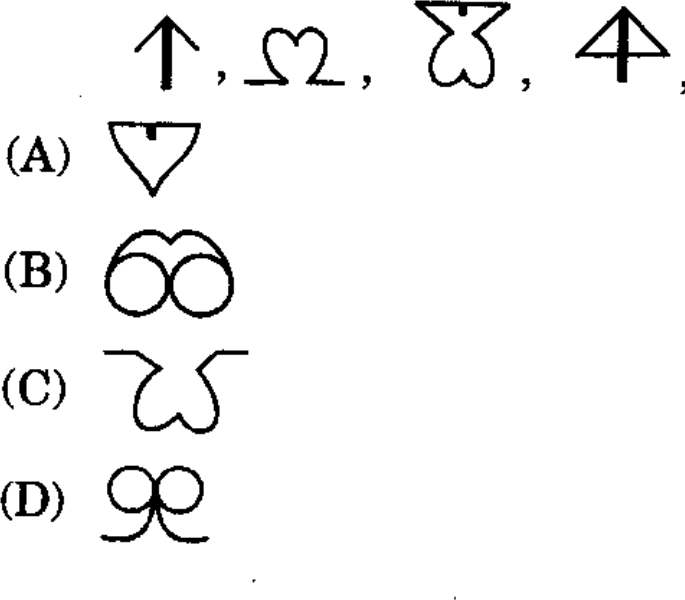
\includegraphics[height=3.6cm]{fig/oct10_q46.png}}
\optsfour{Figure (A)}{Figure (B)}{Figure (C)}{Figure (D)}
\answer{C}{Figure (C)}
\begin{explain}
Each figure is a \textbf{digit joined with its own mirror image}: 1 and its mirror give $\uparrow$, 2 and its mirror give the second shape, then 3 and 4. The next figure must be \textbf{5 joined with its mirror image}, which is figure (C).
\end{explain}
\end{question}

\begin{question}{47}
{If '+' stands for multiplication, '-' stands for division and '*' stands for the power, then the value of [\{(4+3)-2\}*2]-(6*0) is:\par}
\optsfour{30}{25}{35}{20}
\dropped{}
\begin{explain}
Replace the symbols: $[\{(4\times3)\div2\}^2]\div(6^0)=[6^2]\div1=36$.
36 is not among the options, so the agency \textbf{dropped} the question.
\end{explain}
\end{question}

\begin{question}{48}
{Given the correspondence 0 -> -4, 1 -> -3, 2 -> 4, 3 -> 23. Then 3/4 -> ?\par}
\optsfour{520/81}{-341/37}{421/88}{-229/64}
\answer{D}{-229/64}
\begin{explain}
The rule is $x\mapsto x^3-4$: $0-4=-4$, $1-4=-3$, $8-4=4$, $27-4=23$.
\[\left(\tfrac34\right)^3-4=\frac{27}{64}-4=\frac{27-256}{64}=-\frac{229}{64}\]
\end{explain}
\end{question}

\begin{question}{49}
{A person X is taller than Y but shorter than Z. The person V is taller than X but shorter than Z, and W is taller than Y but shorter than X. Then the tallest person will be :\par}
\optsfour{Y}{Z}{V}{X}
\answer{B}{Z}
\begin{explain}
Z $>$ V $>$ X $>$ W $>$ Y, so \textbf{Z} is the tallest.
\end{explain}
\end{question}

\begin{question}{50}
{Make the sequence x, ?, p, l, h. Complete by filling correct answer from the given alternatives.\par}
\optsfour{y}{t}{z}{n}
\answer{B}{t}
\begin{explain}
Positions decrease by 4: x(24), \textbf{t(20)}, p(16), l(12), h(8).
\end{explain}
\end{question}

\begin{question}{51}
{A teacher is teaching in a classroom. The Venn diagram related to school, teacher, classroom and blackboard will be:\par}
\optsfour{\tikz[baseline=-0.5ex,scale=0.3]{\draw (0,0) circle(1.3); \draw (-0.6,0) circle(0.35); \draw (0.6,0) circle(0.4); \draw (0.6,0) circle(0.2);}}{\tikz[baseline=-0.5ex,scale=0.3]{\draw (0,0) circle(1.3); \draw (0,0.7) circle(0.3); \draw (-0.6,-0.3) circle(0.3); \draw (0.6,-0.3) circle(0.3);}}{\tikz[baseline=-0.5ex,scale=0.3]{\draw (0,0) circle(1.3); \draw (0,0) circle(0.85); \draw (-0.3,0) circle(0.25); \draw (0.3,0) circle(0.25);}}{None of (A), (B), (C)}
\answer{C}{\tikz[baseline=-0.5ex,scale=0.3]{\draw (0,0) circle(1.3); \draw (0,0) circle(0.85); \draw (-0.3,0) circle(0.25); \draw (0.3,0) circle(0.25);}}
\begin{explain}
The \textbf{school} contains the \textbf{classroom}, and inside the classroom are the \textbf{teacher} and the \textbf{blackboard} (two separate things). So two small separate circles lie inside the classroom circle, which lies inside the school circle, as in diagram (C).
\end{explain}
\end{question}

\begin{question}{52}
{Fill the correct letter from the given alternatives, in place of question-mark:\\[3pt]
\centering\begin{tabular}{ccc}
\begin{tabular}{|c|c|}\hline C & H\\\hline\multicolumn{2}{|c|}{E}\\\hline R & M\\\hline\end{tabular} &
\begin{tabular}{|c|c|}\hline A & G\\\hline\multicolumn{2}{|c|}{F}\\\hline S & M\\\hline\end{tabular} &
\begin{tabular}{|c|c|}\hline H & J\\\hline\multicolumn{2}{|c|}{?}\\\hline N & L\\\hline\end{tabular}\\
\end{tabular}\par}
\optsfour{C}{K}{B}{O}
\answer{C}{B}
\begin{explain}
The centre letter's position is the difference between the two top letters:
H(8) $-$ C(3) $=5=$ E; G(7) $-$ A(1) $=6=$ F; J(10) $-$ H(8) $=2=$ \textbf{B}.
\end{explain}
\end{question}

\begin{question}{53}
{Put the correct letter in the diagram, from the given alternatives, to replace `?':\\[3pt]
\centering
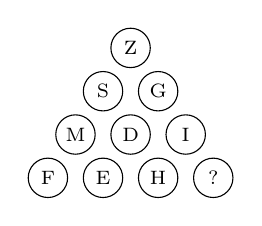
\begin{tikzpicture}[every node/.style={circle,draw,inner sep=1pt,minimum size=5mm,font=\scriptsize}]
\node at (0,0) {Z}; \node at (-0.35,-0.55) {S}; \node at (0.35,-0.55) {G};
\node at (-0.7,-1.1) {M}; \node at (0,-1.1) {D}; \node at (0.7,-1.1) {I};
\node at (-1.05,-1.65) {F}; \node at (-0.35,-1.65) {E}; \node at (0.35,-1.65) {H}; \node at (1.05,-1.65) {?};
\end{tikzpicture}\par}
\optsfour{J}{K}{L}{G}
\answer{D}{G}
\begin{explain}
The positions in every row add up to 26 (Z):
\[\text{S}(19)+\text{G}(7)=26,\quad \text{M}(13)+\text{D}(4)+\text{I}(9)=26\]
\[\text{F}(6)+\text{E}(5)+\text{H}(8)+?=26\Rightarrow ?=7=\mathbf{G}\]
\end{explain}
\end{question}

\begin{question}{54}
{Complete the sequence of squares by choosing the correct figure from the given alternatives:\par}
\qfigure{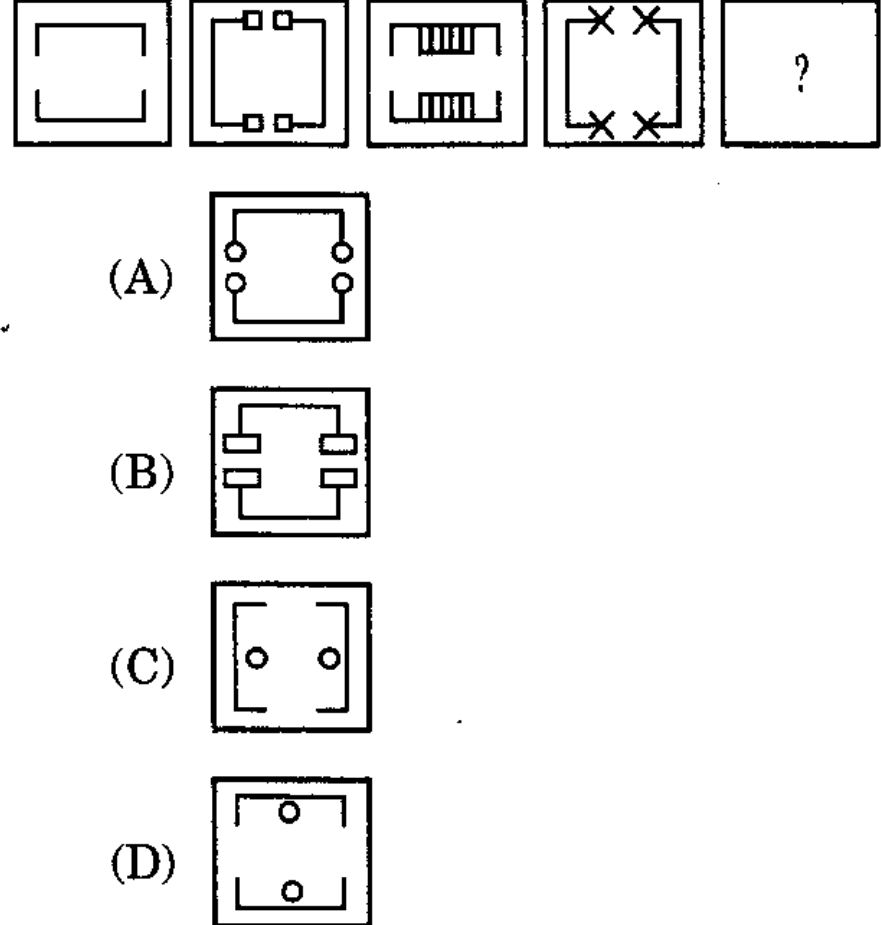
\includegraphics[height=4.6cm]{fig/oct10_q54.png}}
\optsfour{Figure (A)}{Figure (B)}{Figure (C)}{Figure (D)}
\answer{D}{Figure (D)}
\begin{explain}
Two changes alternate. The inner frame alternates between being open on the \emph{sides} and open at the \emph{top and bottom}, and a new decoration appears each time on the \textbf{top and bottom} arms (small squares, hatching, crosses). The fifth figure must again have the frame open like the first and third, with a new element (small circles) on the top and bottom arms, which is figure (D).
\end{explain}
\end{question}

\begin{question}{55}
{Which of the following pollutant gas present in atmosphere is more toxic to human beings ?\par}
\optstwo{Carbon dioxide (CO2)}{Methane (CH4)}{Carbon monoxide (CO)}{Sulphur dioxide (SO2)}
\answer{C}{Carbon monoxide (CO)}
\begin{explain}
\textbf{Carbon monoxide} is the most acutely toxic of these gases. It binds to haemoglobin about 200 times more strongly than oxygen, forming carboxyhaemoglobin and causing suffocation.
\end{explain}
\end{question}

\begin{question}{56}
{Although use of nuclear energy is thought to be pollution free, yet it can pose severe health hazards due to:\par}
\optsone{Nuclear explosion}{Any disaster in nuclear plant}{Unavailability of nuclear waste disposal methods}{Exposure of radiation during normal running of a nuclear plant}
\answer{B}{Any disaster in nuclear plant}
\begin{explain}
Per the key, the chief hazard is \textbf{a disaster in a nuclear plant} (accidents such as Chernobyl 1986 and Fukushima 2011), which releases radioactivity over wide areas.
\end{explain}
\end{question}

\begin{question}{57}
{Green-house effect is increasing due to:\par}
\optsone{Change in atmospheric pressure}{Change in number of green-house gases}{Change in concentration of green-house gases}{Melting of glaciers and dry atmospheric conditions}
\answer{C}{Change in concentration of green-house gases}
\begin{explain}
The greenhouse effect is increasing because the \textbf{concentration} of greenhouse gases (CO$_2$, CH$_4$, N$_2$O) in the atmosphere is rising.
\end{explain}
\end{question}

\begin{question}{58}
{Arrange the following gases in decreasing order of their concentration in atmosphere:\newline (1) Oxygen\newline (2) Nitrogen\newline (3) Carbon dioxide\newline (4) Argon\par}
\optstwo{(2)-(1)-(4)-(3)}{(1)-(2)-(4)-(3)}{(2)-(1)-(3)-(4)}{(2)-(3)-(4)-(1)}
\answer{A}{(2)-(1)-(4)-(3)}
\begin{explain}
Composition of dry air: \textbf{Nitrogen (78\%) $>$ Oxygen (21\%) $>$ Argon (0.93\%) $>$ CO$_2$ ($\approx$0.04\%)}, i.e.\ (2)--(1)--(4)--(3).
\end{explain}
\end{question}

\begin{question}{59}
{Reduction in global warming is possible with:\par}
\optstwo{increased plantation}{conservation of wildlife}{reduction in use of fossil fuel}{(A) and (C)}
\answer{D}{(A) and (C)}
\begin{explain}
Global warming can be reduced by \textbf{increased plantation} (carbon sinks) \textbf{and reduced use of fossil fuels} (fewer emissions), i.e.\ (A) and (C).
\end{explain}
\end{question}

\begin{question}{60}
{Which is the second most important green-house gas besides CO2 responsible for global warming?\par}
\optstwo{Methane}{Chlorofluoro carbon (CFC)}{Nitrous oxide}{Ozone}
\answer{B}{Chlorofluoro carbon (CFC)}
\begin{explain}
Per the key, after CO$_2$ the important greenhouse gas named is \textbf{chlorofluorocarbons (CFCs)}, which have a global-warming potential thousands of times that of CO$_2$.
\tip{By total contribution to warming, methane is usually ranked second after CO$_2$; CFCs are notable for their very high GWP per molecule.}
\end{explain}
\end{question}
